


\clearpage

\section{Yuxtaposición hogar | hospital}

La ubicación actual del hospital es resultado de un proceso histórico que se remonta al siglo XVI, cuando la Corona española ordenó la construcción de hospitales para atender tanto a nativos como a españoles. El primer hospital de Santafé, inicialmente denominado San Pedro, de Jesús, María y José, tuvo dos ubicaciones previas. La primera, como señala \parencite{Romero1994}, se estableció cuando \enquote{Fray Juan de los Barrios y Toledo otorgó escritura pública [...] donando unas casas de su propiedad situadas en la calle de San Felipe (hoy carrera sexta)}, exactamente detrás de la catedral primada, donde funcionaba con apenas doce camas. Posteriormente, en 1723, \enquote{con el producto de la venta de varias casas que pertenecían al Hospital, desde su primera fundación, y con buena parte de las limosnas recibidas, se inició la construcción de la nueva sede bajo la dirección de Fray Pedro Pablo de Villamar} en la calle San Miguel, actual ubicación entre carreras novena y décima con calles once y doce de Bogotá. Finalmente, la institución fue trasladada a los predios del \enquote{Molino de la Hortua}, una finca propiedad de José Domingo Ospina, donde permanece hasta la actualidad.

% Nuevo párrafo sugerido: 
% La arquitectura del hospital refleja una dualidad entre lo institucional y lo doméstico, donde los espacios fueron apropiados por sus habitantes como lugares de vida y trabajo simultáneamente. Esta yuxtaposición entre hogar y hospital se materializa en los jardines interiores, las zonas comunes y las adaptaciones espaciales realizadas por el personal médico y administrativo que habitó el complejo.

\clearpage
\begin{figure}[h!]
    \centering
    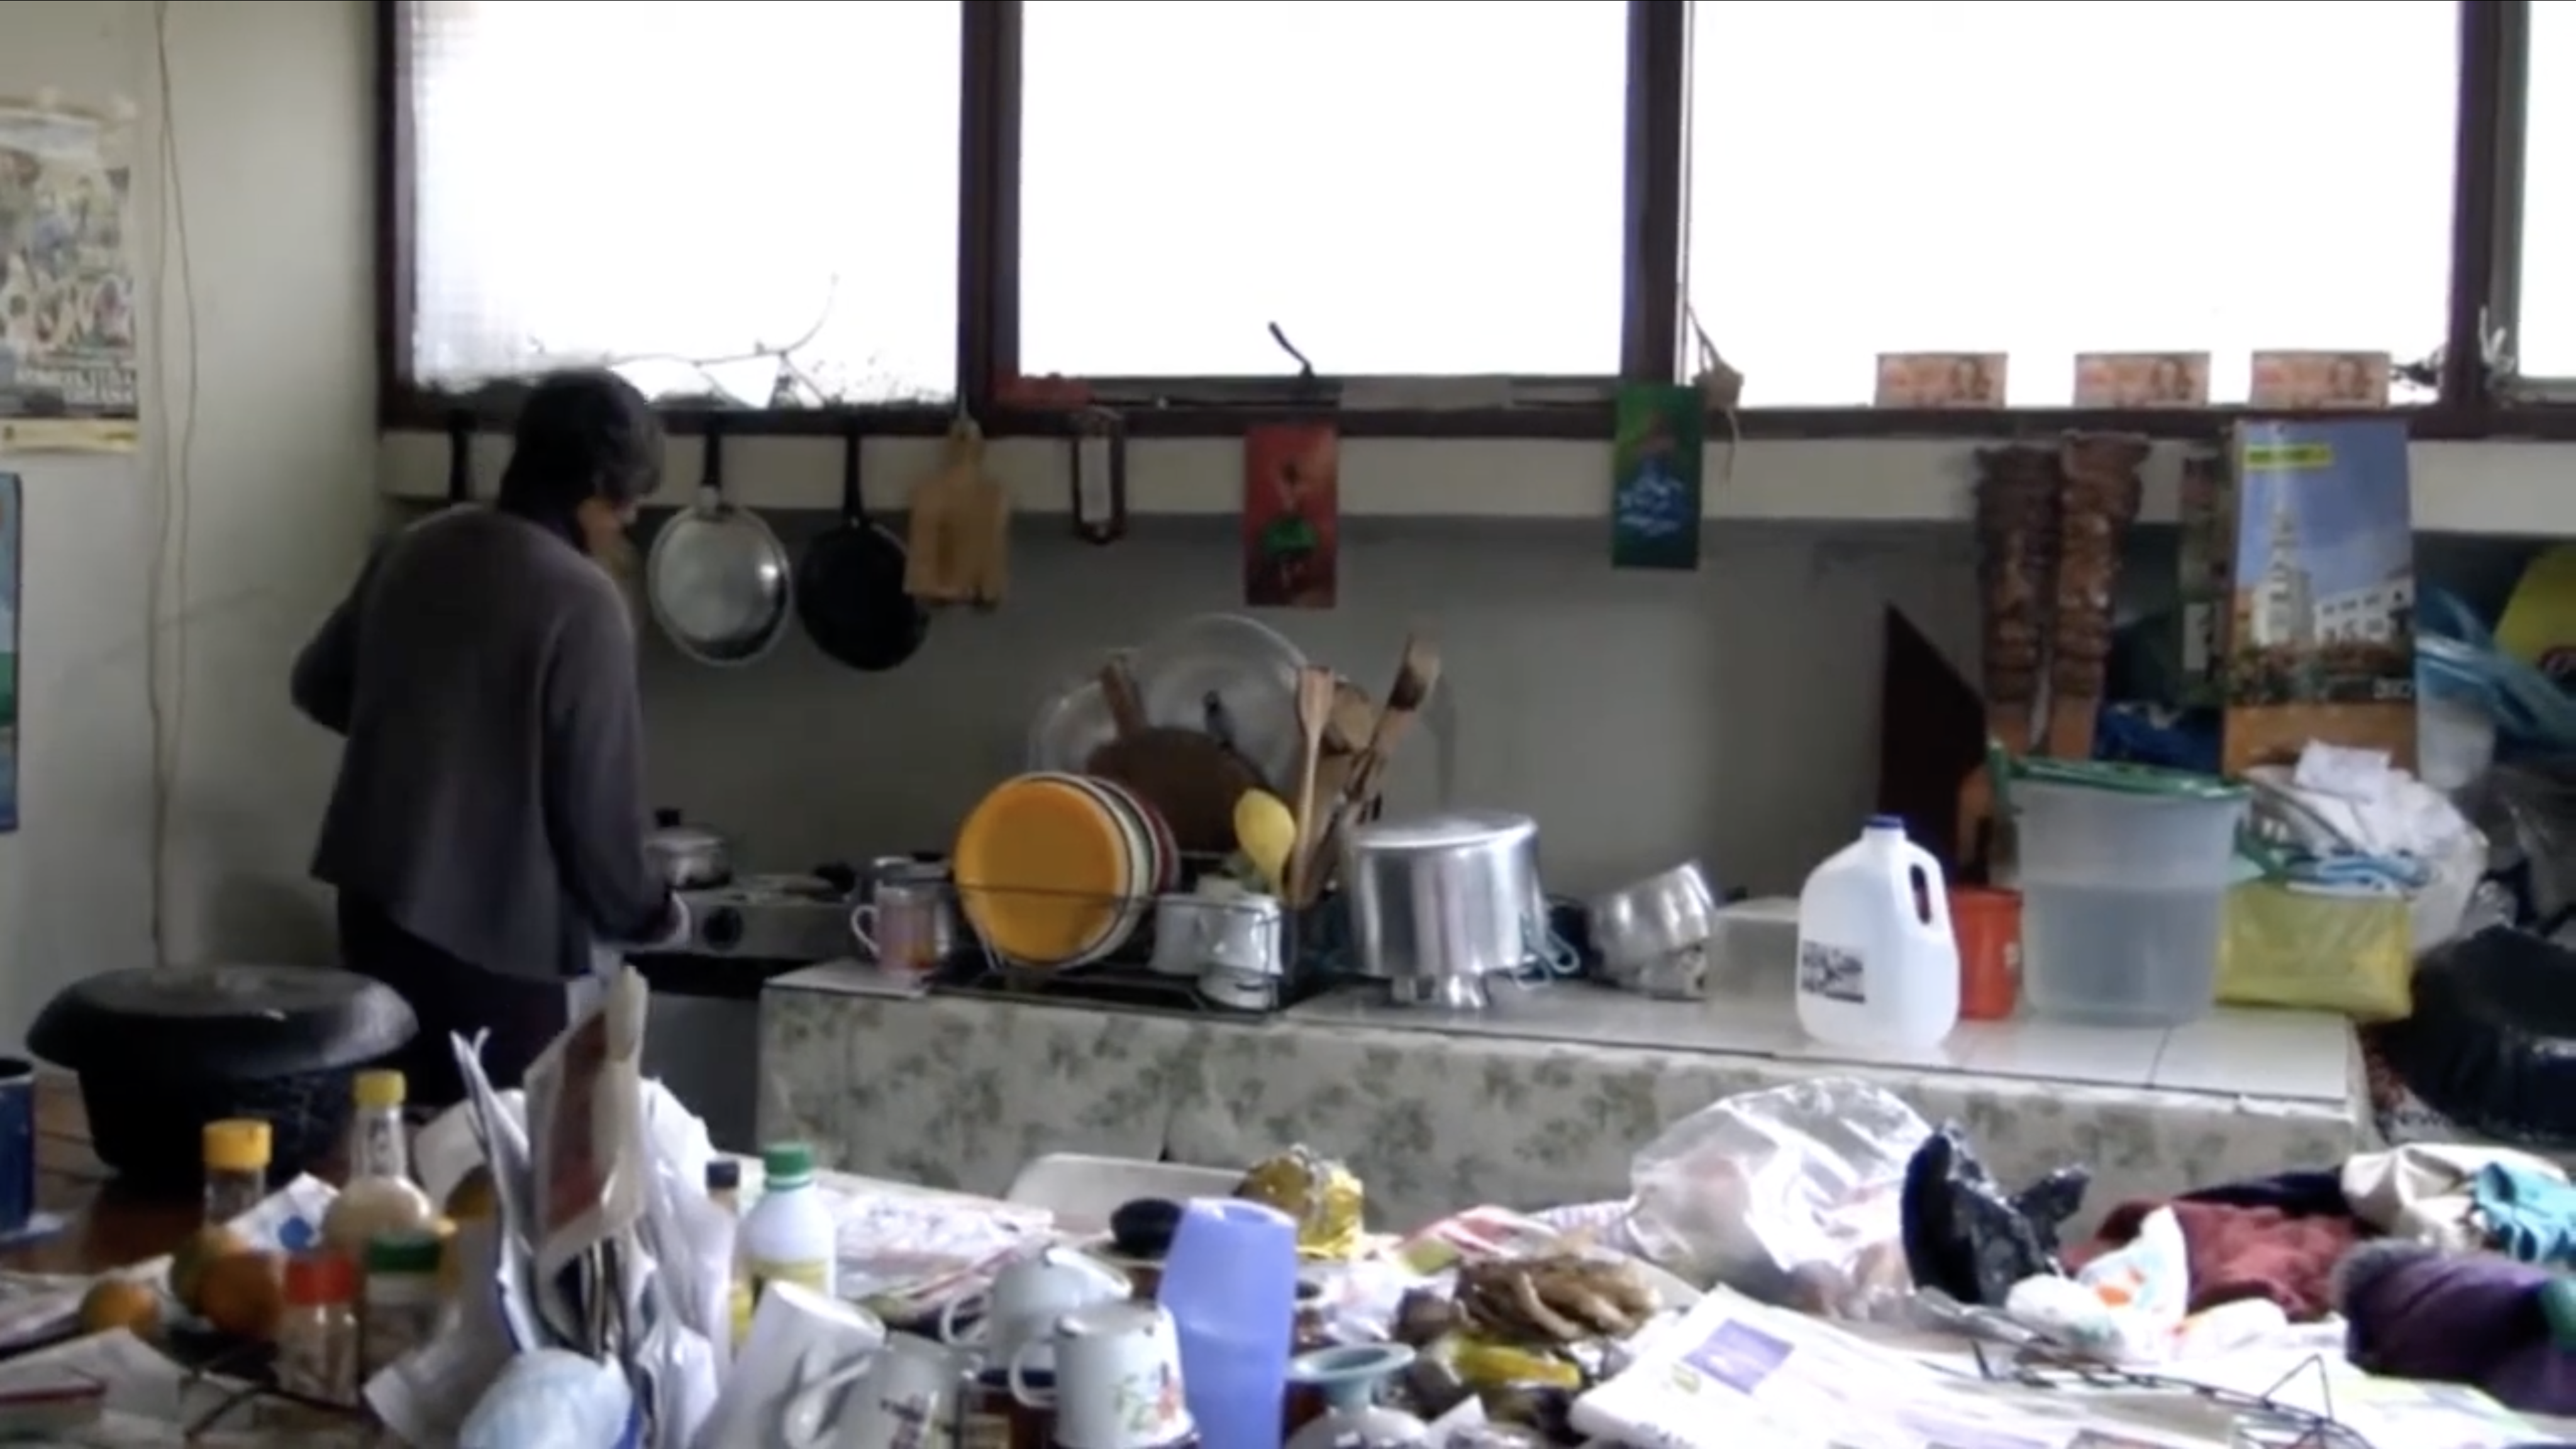
\includegraphics[width=\textwidth]{AlaDeriva_diaz2016_fotograma-00-34-25.png}
    \caption{AlaDeriva diaz2016 fotograma 00:34:25}
    \label{fig:AlaDeriva_diaz2016_fotograma_00_34_25}
\end{figure}

Cocina de tamaño medio, con una ventana grande que ocupa casi toda una pared. La luz natural entra por la ventana, creando sombras y contrastes en los objetos. Una persona de espaldas cocinando en una estufa. Una mesa grande cubierta de objetos, incluyendo platos sucios, bolsas, botellas y papeles. En las paredes hay cuadros y utensilios de cocina colgados. Una mesa en primer plano llena de objetos. La encimera al fondo está llena de utensilios de cocina. \parencite[fotograma: 00:34:25]{AlaDeriva_diaz2016}

\clearpage
\begin{figure}[h!]
    \centering
    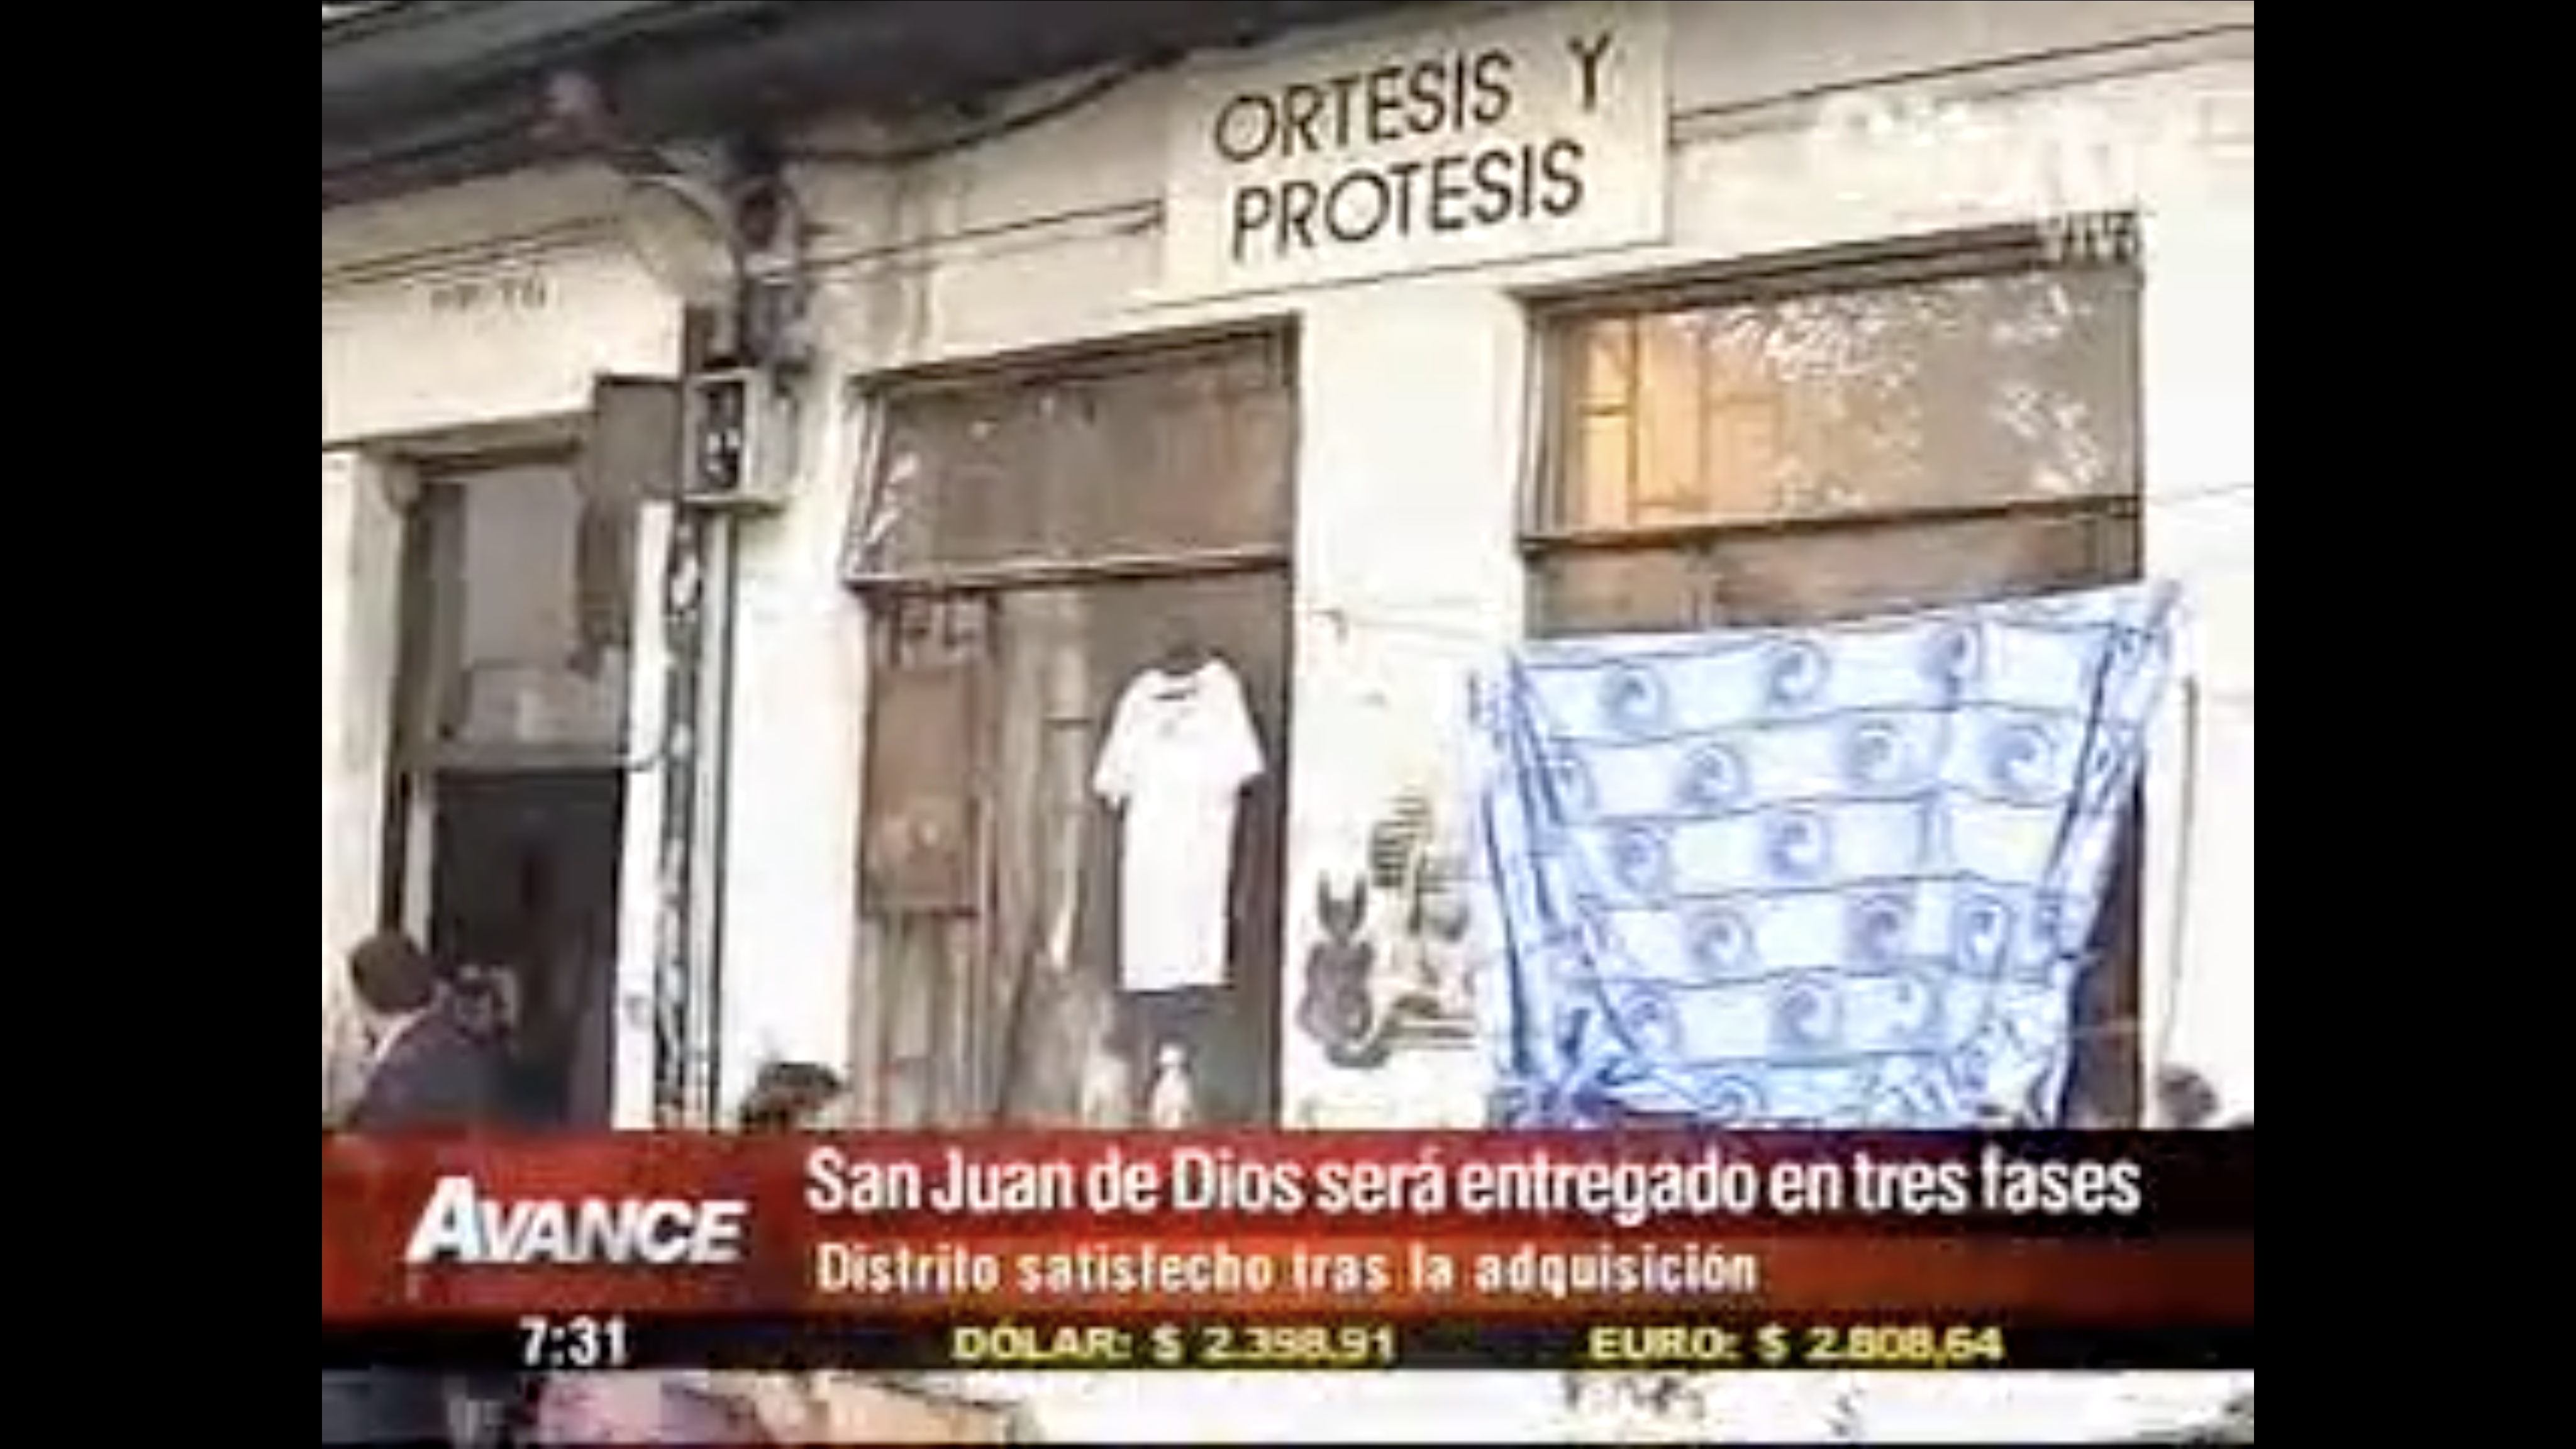
\includegraphics[width=\textwidth]{Citytv_junio2015_fotograma-00-00-16.png}
    \caption{Citytv junio2015 fotograma 00:00:16}
    \label{fig:Citytv_junio2015_fotograma_00_00_16}
\end{figure}

Fachada de un edificio con el letrero `ORTESIS Y PROTESIS'. Hay dos ventanas visibles: una parcialmente cubierta con plástico y una prenda blanca colgando, mientras que la otra tiene una tela clara con patrones color azul. Un cintillo de noticias rojo indica: "San Juan de Dios será entregado en tres fases" y "Distrito satisfecho tras la adquisición", mostrando además la hora 7:31 y los valores del dólar y el euro. Algunas personas aparecen parcialmente visibles en la esquina inferior izquierda. \parencite[fotograma: 00:00:16]{Citytv_junio2015}

\clearpage
\section{Lucha}

Esta institución constituye un hito significativo en la historia de la resistencia social colombiana \parencite{Gongora2013}.

% Nuevo párrafo sugerido:
% La lucha por la preservación del hospital representa no solo una batalla por la infraestructura física, sino por la memoria colectiva y el derecho a la salud pública. Los trabajadores que permanecieron en el hospital después de su cierre transformaron los espacios hospitalarios en símbolos de resistencia, evidenciando la tensión entre el abandono institucional y la persistencia de la comunidad hospitalaria.

\clearpage
\begin{figure}[h!]
    \centering
    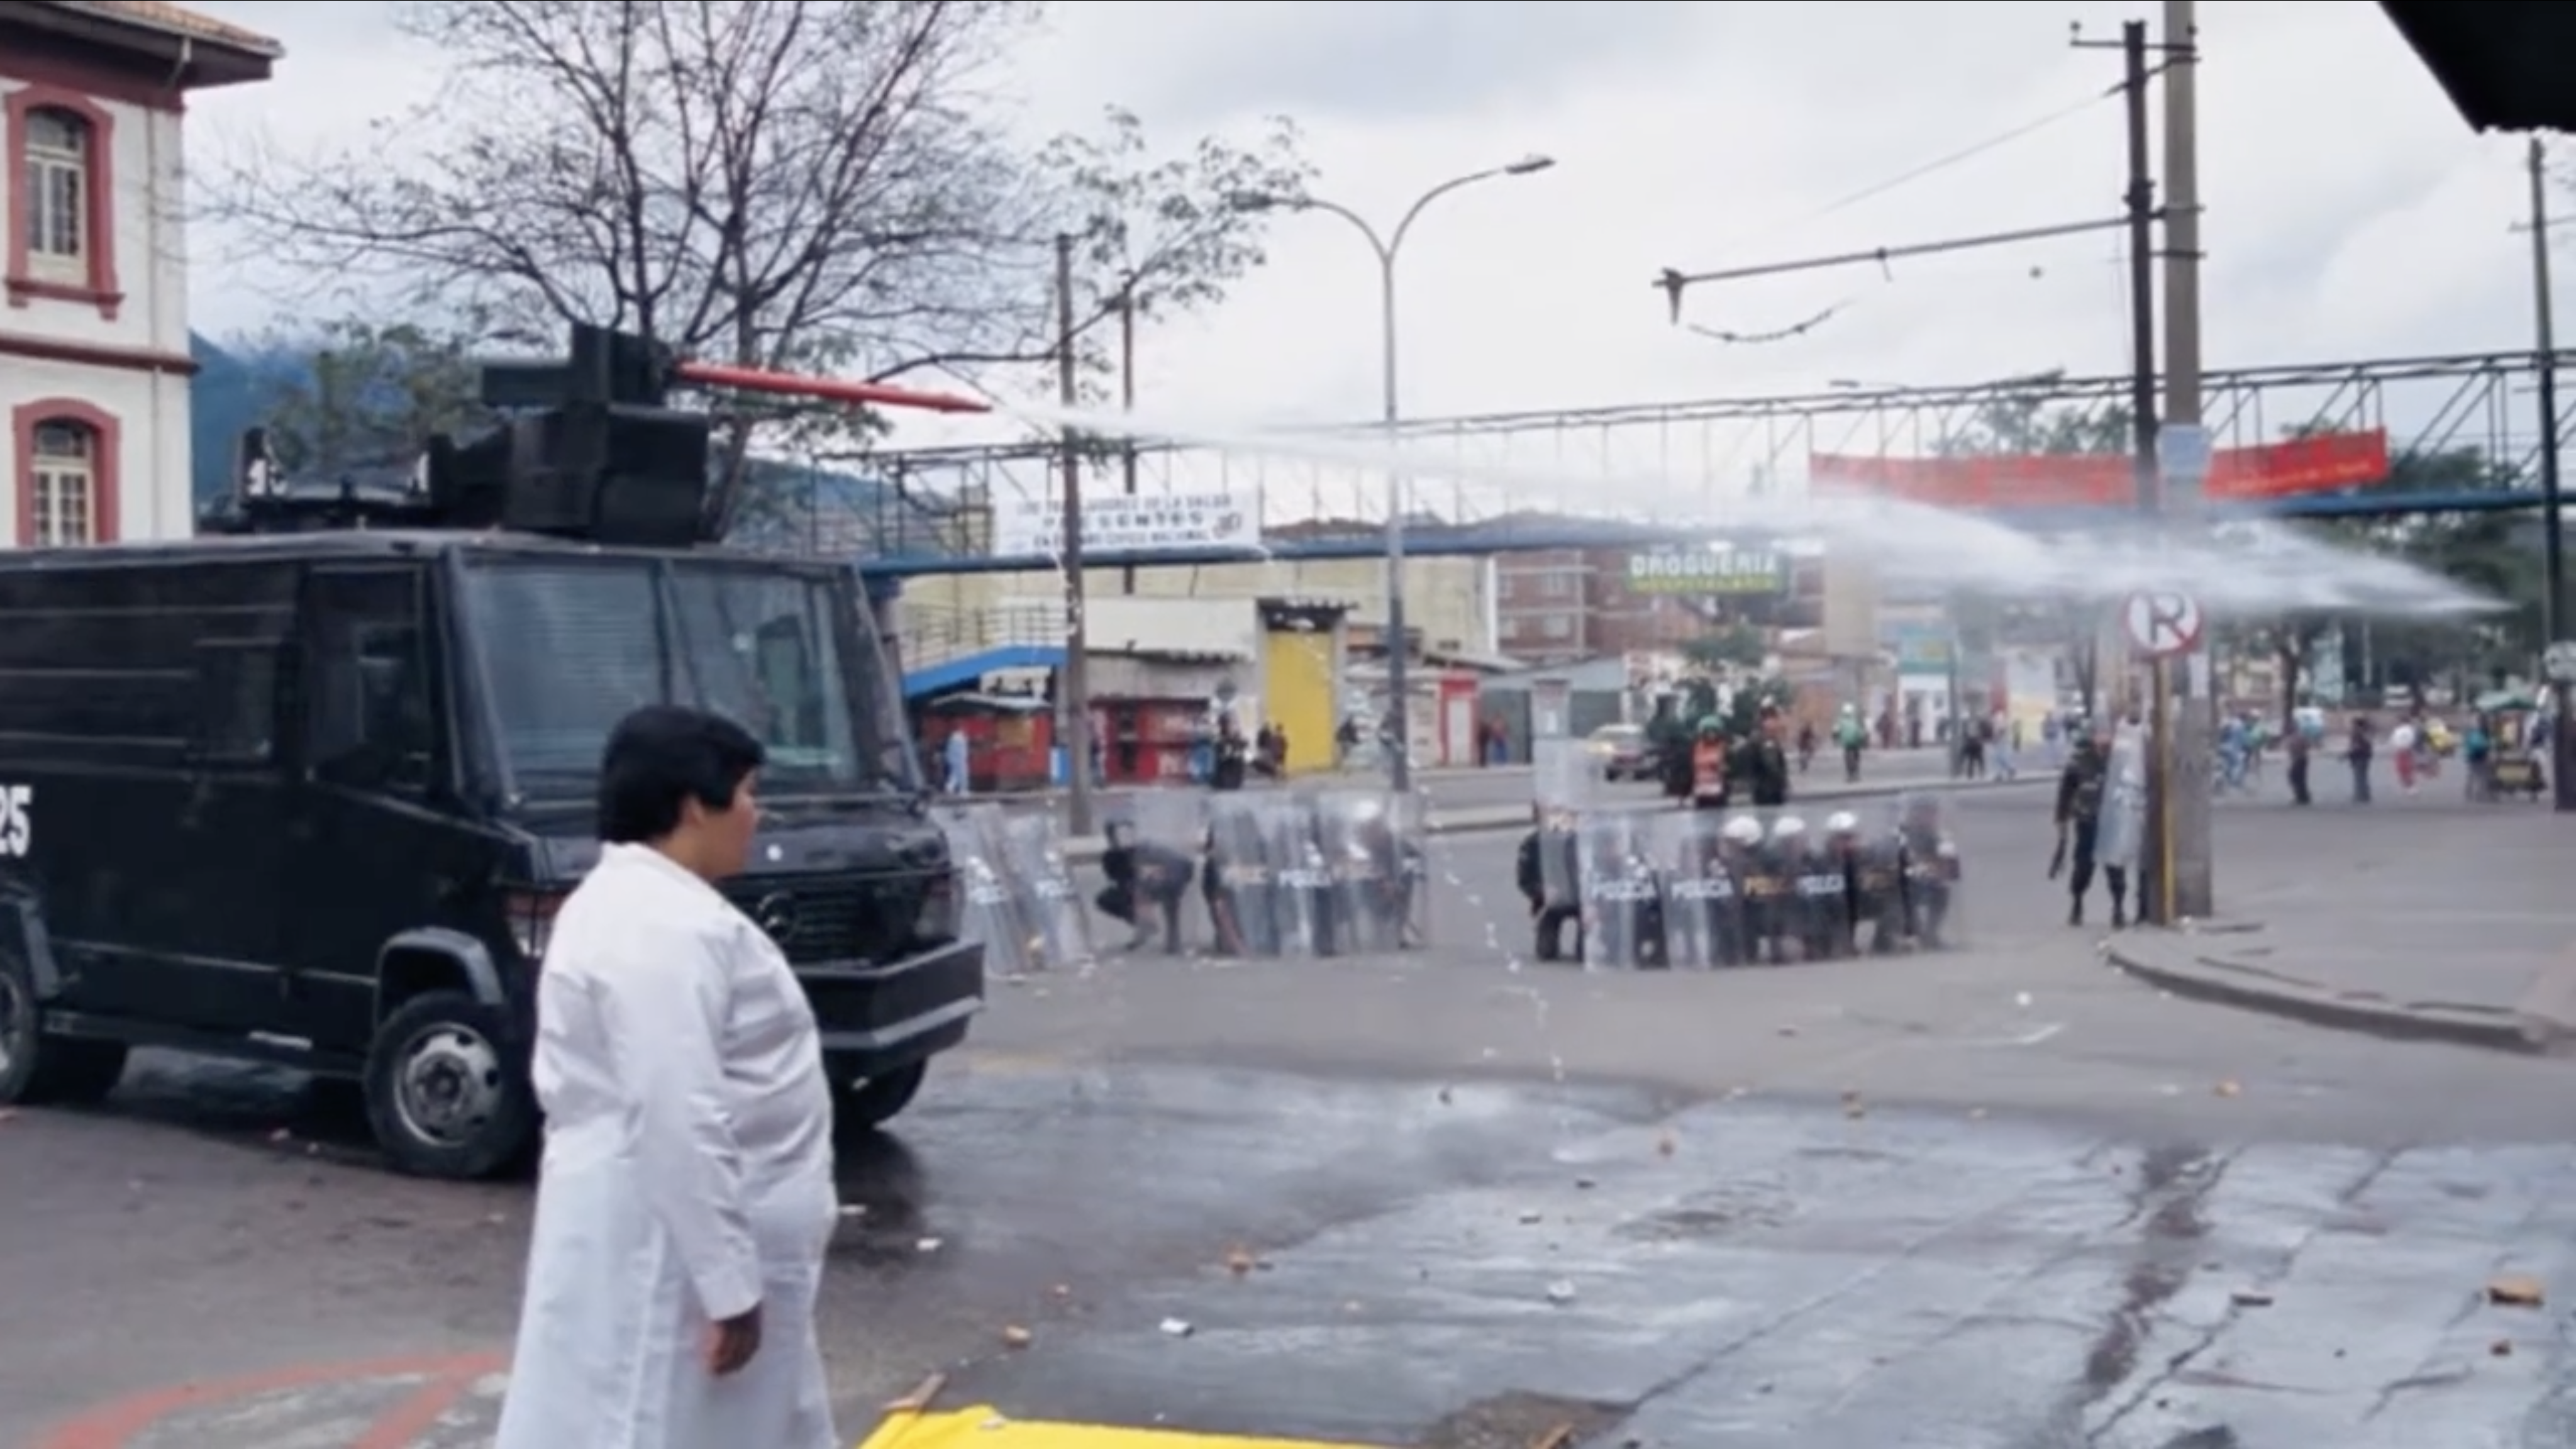
\includegraphics[width=\textwidth]{AlaDeriva_diaz2016_fotograma-00-05-54.png}
    \caption{AlaDeriva diaz2016 fotograma 00:05:54}
    \label{fig:AlaDeriva_diaz2016_fotograma_00_05_54}
\end{figure}

Exterior del HSJD carrera décima vista hacia el sur. Se observa un vehículo blindado negro tipo antimotines con equipo de dispersión de agua en el techo. En primer plano, sobre el pavimento mojado, hay una persona vestida con bata blanca. Al fondo se distingue un grupo de policías con escudos antidisturbios formando una línea, mientras un chorro de agua es disparado hacia la derecha de la escena. \parencite[fotograma: 00:05:54]{AlaDeriva_diaz2016}

\clearpage
\section{Objetos | situaciones icónicas}

El sector se caracteriza por la presencia de importantes símbolos urbanísticos de relevancia histórica local y nacional. En su entorno inmediato se encuentran el parque Tercer Milenio, la iglesia del Voto Nacional y barrios tradicionales como el Policarpa, San Bernardo y Eduardo Santos. Asimismo, el área presenta una notable concentración de instituciones de salud, estableciendo vínculos con el Hospital Santa Clara, La Samaritana y el Hospital de la Misericordia, entre otros. La zona combina usos residenciales y comerciales, con predominio de la industria textil, mecánica y de fabricación de muebles y enseres.

La ubicación actual del hospital es resultado de un proceso histórico que se remonta al siglo XVI, cuando la Corona española ordenó la construcción de hospitales para atender tanto a nativos como a españoles. El primer hospital de Santafé, inicialmente denominado San Pedro, de Jesús, María y José, tuvo dos ubicaciones previas. La primera, como señala \parencite{Romero1994}, se estableció cuando \enquote{Fray Juan de los Barrios y Toledo otorgó escritura pública [...] donando unas casas de su propiedad situadas en la calle de San Felipe (hoy carrera sexta)}, exactamente detrás de la catedral primada, donde funcionaba con apenas doce camas. Posteriormente, en 1723, \enquote{con el producto de la venta de varias casas que pertenecían al Hospital, desde su primera fundación, y con buena parte de las limosnas recibidas, se inició la construcción de la nueva sede bajo la dirección de Fray Pedro Pablo de Villamar} en la calle San Miguel, actual ubicación entre carreras novena y décima con calles once y doce de Bogotá. Finalmente, la institución fue trasladada a los predios del \enquote{Molino de la Hortua}, una finca propiedad de José Domingo Ospina, donde permanece hasta la actualidad.

% Nuevo párrafo sugerido:
% Los objetos y espacios del hospital se han convertido en elementos icónicos que testimonian diferentes momentos históricos de la institución. Desde los instrumentos médicos abandonados hasta los murales y grafitis de protesta, estos elementos materiales constituyen un archivo visual de la transformación del hospital y su significado social a través del tiempo.

\clearpage
\begin{figure}[h!]
    \centering
    \includegraphics[width=\textwidth]{archivoMargarita_6octubre2004.jpg}
    \caption{Archivo Margarita 6 de octubre 2004}
    \label{fig:archivoMargarita_6octubre2004}
\end{figure}

Sala de espera con una fila de asientos blancos de plástico montados sobre una estructura metálica negra. La pared es de color crema claro con algunos elementos montados como un tablero y un teléfono naranja. El piso tiene un patrón geométrico en tonos beige y gris. En la escena hay una persona vestida de negro que mira hacia el suelo a lo que perece ser un marco y cristal rotos. Hay una bicicleta, un balón de fútbol y detrás de la hilera de sillas a la izquierda una puerta con letreros de `SELLADO'.












